\begin{figure}[t]
\centering
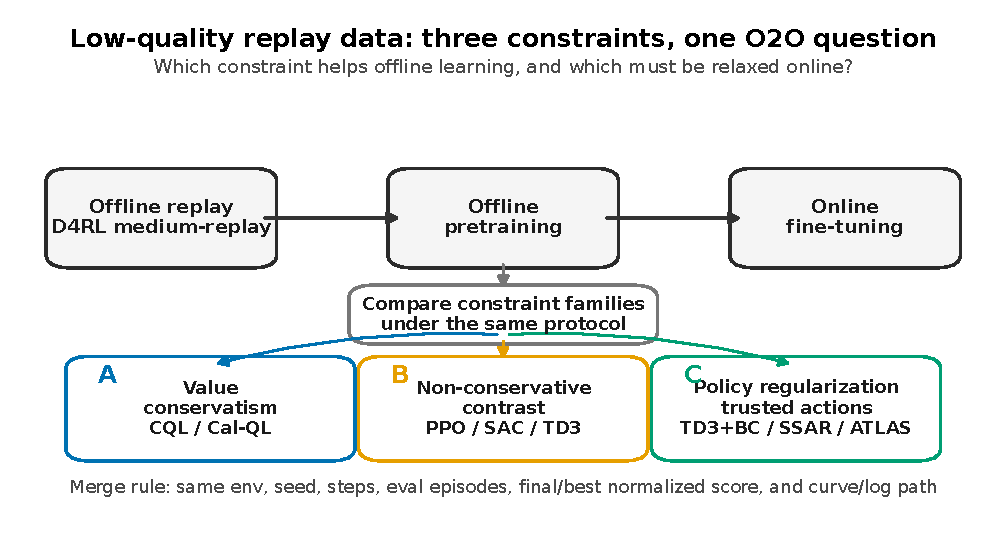
\includegraphics[width=\linewidth]{../figures/fig1_project_story.pdf}
\caption{Project framing. The final report compares three constraint families under one offline-to-online question.}
\label{fig:project-story}
\end{figure}

\begin{figure}[t]
\centering
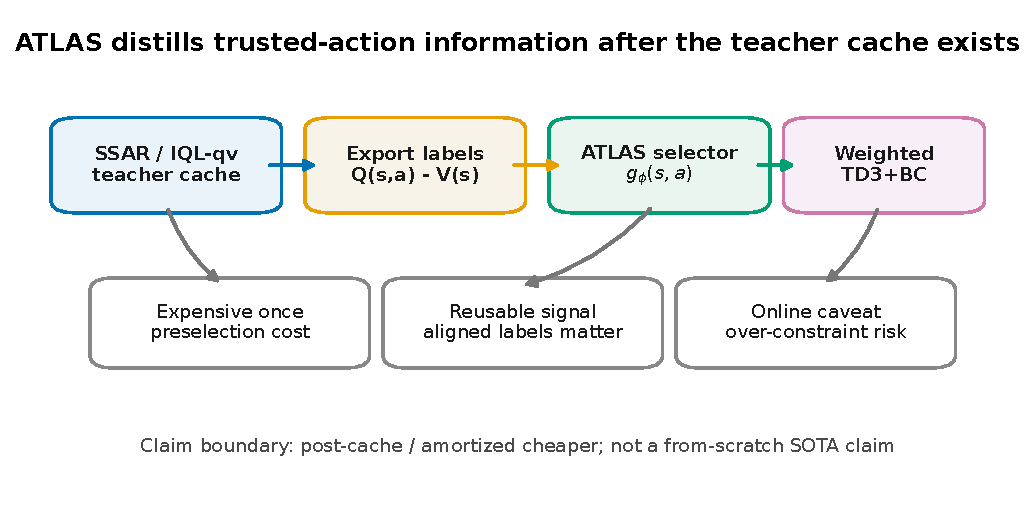
\includegraphics[width=\linewidth]{../figures/fig2_atlas_mechanism.pdf}
\caption{ATLAS mechanism. ATLAS distills trusted-action labels from a cached SSAR/IQL-qv teacher and uses them for weighted TD3+BC-style learning.}
\label{fig:atlas-mechanism}
\end{figure}

\begin{figure}[t]
\centering
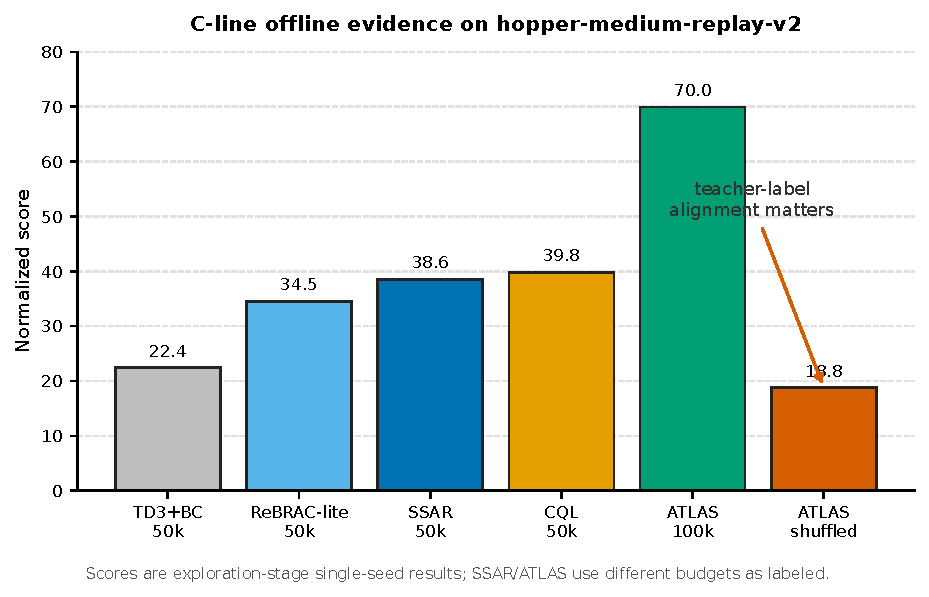
\includegraphics[width=0.92\linewidth]{../figures/fig3_offline_results.pdf}
\caption{C-line offline evidence on \texttt{hopper-medium-replay-v2}. Aligned ATLAS labels improve the offline endpoint, while shuffled labels collapse.}
\label{fig:offline-results}
\end{figure}

\begin{figure}[t]
\centering
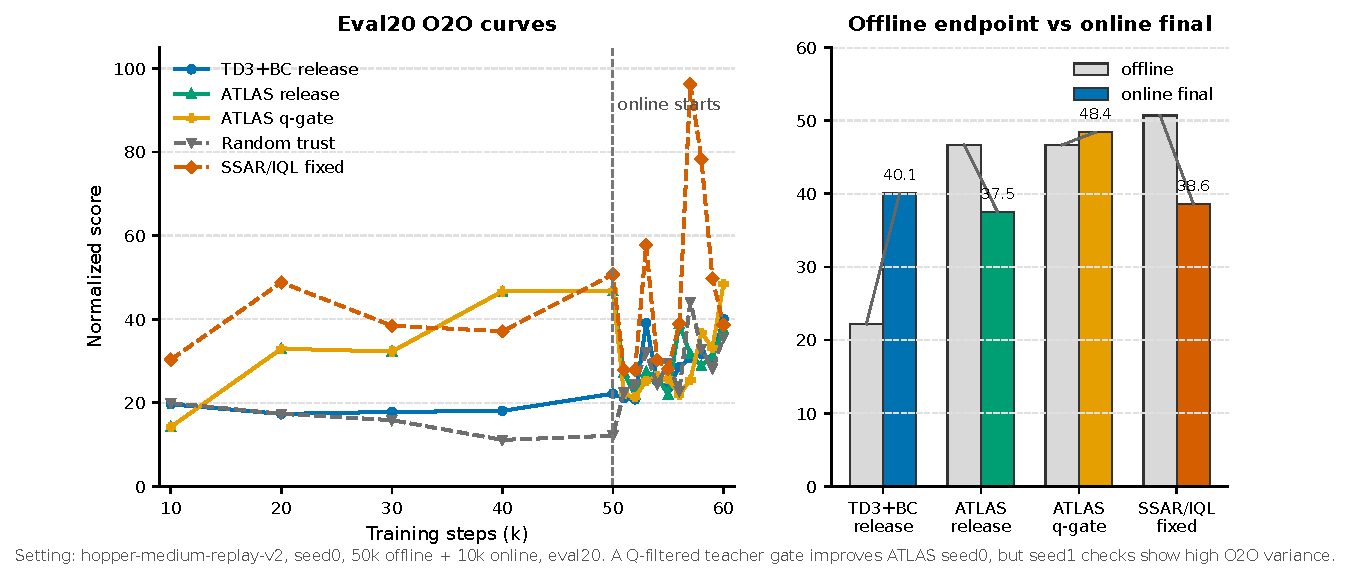
\includegraphics[width=0.92\linewidth]{../figures/fig4_o2o_curve.pdf}
\caption{P0 offline-to-online eval20 panel. Stronger teacher labels improve offline endpoints but do not improve final online score under the current online regularizer.}
\label{fig:o2o-curve}
\end{figure}
